% Artigo único (Lab03), compacto para o limite de 10 páginas. Estrutura do enunciado (seção 8) com os itens do
% modelo geral de relatório (desafios, decisões, etapas, ferramentas, tabela de métricas, contribuições, conclusão).
% Overleaf: abrir o projeto do template SBC, substituir o main.tex por este arquivo e enviar a pasta figuras/ e o
% referencias.bib. Os arquivos sbc-template.sty e sbc.bst vêm do template.
\documentclass[12pt]{article}

\usepackage{sbc-template}
\usepackage{graphicx,url}
\usepackage[brazil]{babel}
\usepackage[utf8]{inputenc}
\usepackage[T1]{fontenc}
\usepackage{booktabs,array}

\sloppy
% espaço mais enxuto ao redor de figuras e tabelas, para caber no limite de páginas
\setlength{\textfloatsep}{8pt plus 2pt minus 2pt}
\setlength{\floatsep}{6pt plus 2pt minus 2pt}
\setlength{\abovecaptionskip}{4pt}

\title{Mineração de Métricas DORA em Repositórios Open-Source que Usam GitHub Actions}

\author{Arthur Henrique Santana Pedra\inst{1}, Gabriel Felipe Santos de Souza\inst{1}, Pedro Porto Ramalho\inst{1}}

\address{Pontifícia Universidade Católica de Minas Gerais (PUC Minas) \\
  Curso de Engenharia de Software
  \email{arthurpedrasantana@gmail.com, gf.22142@gmail.com, portorpedro@gmail.com}
}

\begin{document}

\maketitle

\begin{abstract}
DORA metrics are the standard for measuring software delivery performance, but GitHub records neither production deploys nor failures. We compute the four metrics from proxies (published releases and GitHub Actions runs) for 300 popular open-source repositories over 12 months, and measure how much the results depend on the definitions adopted. Three raters validated the corrective-release heuristic (Fleiss' kappa 0.65; F1 0.73), and 24\% to 26\% of the repositories change DORA category across three combinations of operational definitions. The delivery-based failure rate grows with deploy frequency ($\rho=0.48$), largely as an artifact of the proxy, and repository age is the factor most associated with lead time. Per-metric classifications are sensitive to the definitions, and release frequency measures version publishing rather than production deploys.
\end{abstract}

\begin{resumo}
As métricas DORA são o padrão para medir o desempenho de entrega de software, mas o GitHub não registra deploys nem falhas em produção. Calculamos as quatro métricas a partir de proxies (releases publicadas e execuções do GitHub Actions) em 300 repositórios populares de código aberto, ao longo de 12 meses, e medimos o quanto os resultados dependem das definições adotadas. Três avaliadores validaram a heurística de release corretiva (kappa de Fleiss de 0,65; F1 de 0,73), e de 24\% a 26\% dos repositórios mudam de categoria DORA entre três combinações de definições operacionais. A taxa de falha por entrega cresce com a frequência de deploy ($\rho=0{,}48$), em boa parte como efeito do proxy, e a idade do repositório é o fator mais associado ao lead time. A classificação por métrica é sensível às definições, e a frequência de releases mede a publicação de versões, não o deploy em produção.
\end{resumo}

\section{Introdução}
\label{sec:intro}

As métricas DORA (\emph{DevOps Research and Assessment})~\cite{forsgren2018,dora_fourkeys} combinam velocidade (frequência de deploys e \emph{lead time} do commit até a entrega) e estabilidade (taxa de falha das mudanças, CFR, e tempo de recuperação), e sua tese é que velocidade e estabilidade não são um \emph{trade-off}. O GitHub, porém, só registra releases, execuções de CI e commits. Medimos DORA, então, por \textbf{proxies}: uma release publicada vale um deploy, e uma execução de CI com falha vale uma falha. Proxies enganam: uma biblioteca que publica uma versão por mês não coloca nada em produção, e um teste instável não é um incidente percebido por ninguém fora do projeto.

Mineramos as métricas de 300 repositórios populares (mais de 1.000 estrelas) com GitHub Actions, em 12 meses, e perguntamos \textbf{o quanto se pode confiar nelas}: (i) validamos os critérios automáticos contra o julgamento de três avaliadores, em uma amostra-ouro de 60 repositórios, e (ii) medimos a sensibilidade da classificação (Elite, High, Medium, Low) às definições. As questões: RQ 01, frequência de deploy; RQ 02, lead time; RQ 03, taxa de falha; RQ 04, recuperação; RQ 05, frequência e taxa de falha; RQ 06, características associadas ao desempenho; RQ 07, sensibilidade da classificação; RQ 08 (bônus), \emph{rework rate}.

\paragraph{Hipóteses.} Escritas antes da coleta e confrontadas com os resultados na Seção~\ref{sec:discussao}.
\begin{itemize}\setlength{\itemsep}{0pt}\setlength{\parskip}{0pt}
\item \textbf{H1.} Frequência mediana abaixo de uma release por semana, maioria \emph{Medium} e cauda longa (uma release reúne muitas mudanças).
\item \textbf{H2.} Lead time por commit (b) de dias a poucas semanas; por release (a) sistematicamente maior, com muitos repositórios acima de 30 dias (um commit antigo basta para inflá-lo).
\item \textbf{H3.} CFR de CI (a) com mediana de 10\% a 25\% (testes instáveis, workflows auxiliares); CFR de entrega (b) menor, a maioria abaixo de 15\%, e correlação fraca entre (a) e (b).
\item \textbf{H4.} Recuperação mediana de 1 h a 1 dia (falha no default branch é visível), com cauda longa e poucos episódios censurados.
\item \textbf{H5.} Correlação entre frequência e CFR (a) fraca ou nula, talvez levemente negativa; com o CFR (b), fraca e positiva, em parte artefato do proxy.
\item \textbf{H6.} (i) Mais contribuidores, maior frequência e menor lead time; (ii) bibliotecas publicam menos e têm lead time maior; (iii) JavaScript/TypeScript, Go e Rust publicam mais que C/C++ e Java; (iv) projetos mais antigos têm lead time maior. Efeitos pequenos a médios e poucas diferenças após Holm.
\item \textbf{H7.} Ao menos 30\% dos repositórios mudam de categoria geral entre C1 e uma alternativa, com kappa ponderado de 0,4 a 0,6, sobretudo com tags e pré-releases, e a maioria entre categorias vizinhas.
\item \textbf{H8.} \emph{Rework rate} maior que o CFR (b), da mesma ordem (10\% a 25\%) e fortemente correlacionada com ele.
\end{itemize}

\section{Metodologia}
\label{sec:metodologia}

\subsection{Dados, ferramentas e seleção}

Os dados vêm das APIs REST do GitHub, coletadas em 14 e 15 de outubro de 2026 por um pipeline próprio em Python (\texttt{requests}, sem bibliotecas prontas de acesso à API), com um único comando, cache em disco e retomada, espera pelo limite de requisições e \emph{backoff} exponencial. As análises usam pandas, SciPy, statsmodels e scikit-learn; os testes (pytest, 100\% de cobertura do módulo de métricas) rodam no GitHub Actions; e o trabalho é organizado no GitHub Projects. A janela vai de 01/10/2025 a 30/09/2026 (UTC), no default branch.

Os candidatos têm mais de 1.000 estrelas, não são arquivados nem espelhos e são avaliados em ordem decrescente de estrelas, em faixas, até chegar a 300 repositórios. Dos 707 avaliados, 68 não usam GitHub Actions, 293 têm menos de 5 releases e 46 têm menos de 50 runs válidos na janela, o que deixa 300. A amostra reúne os elegíveis mais populares (todos com 40.642 estrelas ou mais, mediana de 62.121).

\subsection{Principais desafios e decisões}

Os desafios foram: (i) o teto de 1.000 resultados por consulta, que exigiu fatiar a busca por estrelas e subdividir os runs até frações de dia (sem isso, 12 candidatos com mais de 1.000 runs num dia seriam descartados, como \texttt{pytorch/pytorch}); (ii) o limite de requisições (os primeiros 100 repositórios levaram cerca de 12 h), o que tornou cache e retomada essenciais; (iii) o lead time com linhas de versão paralelas: comparar a \texttt{godot 3.6.3} com a 4.7.2 dava 9.545 commits, e por isso comparamos cada release com a anterior da mesma linha de versão (28 commits); e (iv) a rotulagem manual, circular na primeira rodada (Seção~\ref{sec:validacao}). Mantivemos a heurística v1, já em uso, pois atinge a meta de F1 e a v4 só a supera por 3 pontos.

\subsection{Tabela de métricas e definições operacionais}
\label{sec:definicoes}

A Tabela~\ref{tab:metricas} resume as métricas. Um \emph{deploy} é uma release publicada (não rascunho nem pré-release); a data de um commit é \texttt{commit.author.date}; os runs de CI são os disparados por \texttt{push}, com \texttt{success} como sucesso, \texttt{failure}, \texttt{timed\_out} e \texttt{startup\_failure} como falha e as demais conclusões ignoradas. A classificação geral é a mediana das quatro notas (Elite $=4$, \ldots, Low $=1$), arredondada para baixo, pelos cortes fixos da disciplina. C1 (referência) usa release, lead time (a) e CFR (a); C2, release e pré-release, lead time (b) e CFR (b); C3, tag, lead time (b) e CFR (a). Resumimos tudo por mediana e intervalo interquartil (IQR).

\begin{table}[!t]
\centering
\footnotesize
\setlength{\tabcolsep}{3pt}
\caption{Métricas e definições operacionais.}
\label{tab:metricas}
\begin{tabular}{>{\raggedright\arraybackslash}p{1.0cm}>{\raggedright\arraybackslash}p{2.7cm}>{\raggedright\arraybackslash}p{8.4cm}>{\raggedright\arraybackslash}p{2.8cm}}
\toprule
RQ & Métrica & Definição operacional & Fonte \\
\midrule
01 & Frequência & Releases publicadas na janela divididas por 52,1 semanas (releases/semana). & \texttt{/releases} \\
02 & Lead time & (a) release menos o commit mais antigo dela; (b) release menos cada commit; mediana por repositório, em horas. & \texttt{/compare} \\
03 & CFR (a) & Falhas divididas por falhas mais sucessos de CI. & \texttt{/actions/runs} \\
03 & CFR (b) & Releases seguidas, em até 7 dias, por uma release corretiva (heurística v1: muda só o \emph{patch} e há commit com \texttt{fix}, \texttt{hotfix}, \texttt{bugfix} ou \texttt{revert}), sobre as avaliadas; as dos últimos 7 dias são censuradas. & \texttt{/releases}, \texttt{/compare} \\
04 & Recuperação & Da primeira falha após um sucesso até o próximo sucesso do mesmo workflow, em horas; episódios sem sucesso são censurados e reportados como proporção. & \texttt{/actions/runs} \\
05--06 & Spearman, Kruskal-Wallis & $\rho$ entre frequência e CFR; Kruskal-Wallis entre grupos com correção de Holm e $\varepsilon^2=H/(n-1)$. & \texttt{metrics.csv} \\
07 & Classificação & Categoria geral em C1, C2 e C3; kappa ponderado entre pares. & cortes fixos \\
08 & \emph{Rework rate} & Releases corretivas (v1) divididas por todas as releases. & \texttt{/compare} \\
\bottomrule
\end{tabular}
\end{table}

\subsection{Validação manual e heurística de release corretiva}
\label{sec:validacao}

O CFR (b) depende de uma heurística de release corretiva (objetivo principal: corrigir um defeito recente). Para medir seu erro, sorteamos 60 repositórios (semente 42), de um subconjunto de 100 da amostra, e 5 releases de cada, totalizando 300. Três avaliadores rotularam, cada um sozinho e sem ver a saída da heurística, o tipo do projeto, se as releases são entregas reais ao usuário e se cada release é corretiva. A primeira rodada foi descartada: dois avaliadores coincidiam com a regra do número de versão em 95\% e 98\% das releases, o que tornaria a validação circular. Na segunda, a dimensão \emph{entrega real} teve $\kappa=-0{,}009$ por critério ambíguo, e os três a refizeram, sozinhos, com uma regra escrita igual para todos.

Medimos a concordância com o kappa de Fleiss~\cite{fleiss1971} sobre os votos originais, interpretado pela escala de Landis e Koch~\cite{landis1977}: $\kappa=0{,}648$ (substancial) em corretiva, $0{,}827$ (quase perfeita) no tipo do projeto e $0{,}372$ (razoável) em entrega real. Este é baixo apesar de 87\% de concordância, porque quase todos os repositórios são \emph{sim} (o paradoxo do kappa~\cite{feinstein1990}); o AC1 de Gwet~\cite{gwet2008} foi de 0,851. Não houve empates 1-1-1, e o consenso é a maioria simples.

Comparamos quatro variantes da heurística com o consenso (133 corretivas em 300), com meta de F1 $\geq 0{,}70$: v1, \emph{patch} e correção (precisão 0,68; \emph{recall} 0,78; F1 \textbf{0,73}); v2, \emph{patch} ou correção (F1 0,63); v3, só correção (0,60); e v4, só \emph{patch} (0,76). Como os avaliadores usaram limiares diferentes (um marcou 165 releases como corretivas, contra 112 e 116), repetimos a avaliação com outras referências: o F1 da v1 é 0,72 nos 222 casos unânimes e 0,76 se basta um avaliador marcar, mas \textbf{0,56} se exige os três. A conclusão de que a v1 atinge a meta não se sustenta sob a referência mais estrita.

\subsection{Etapas e contribuições além do enunciado}

O trabalho seguiu quatro sprints (Tabela~\ref{tab:etapas}), em um quadro do GitHub Projects com as colunas Todo, In Progress e Done. Além do enunciado, contribuímos com: a subdivisão dos runs até frações de dia, para não descartar os projetos mais ativos; a escolha da release anterior da mesma linha de versão; a avaliação do F1 sob diferentes referências e o AC1 como complemento ao kappa (Seção~\ref{sec:validacao}); a segunda passada com regra escrita na entrega real; e um script que compara uma replicação com o CSV original.

\begin{table}[!t]
\centering
\footnotesize
\setlength{\tabcolsep}{3pt}
\caption{Sprints, entregas e responsáveis (nº das issues).}
\label{tab:etapas}
\begin{tabular}{>{\raggedright\arraybackslash}p{1.2cm}>{\raggedright\arraybackslash}p{14.4cm}}
\toprule
Sprint & Entregas por responsável (nº da issue) \\
\midrule
S01 & \textbf{Arthur:} cliente REST com cache e rate limit (\#17), README e dicionário (\#20), CI (\#22). \textbf{Pedro:} métricas e testes (\#18), introdução e hipóteses (\#21). \textbf{Gabriel:} seleção, funil e coleta de 100 repositórios (\#19). \\
S02 & \textbf{Pedro:} coleta de 300 repositórios e \texttt{metrics.csv} (\#28). \textbf{Gabriel:} amostra-ouro, kappa e consenso (\#30). \textbf{Arthur:} heurística corretiva e sua validação (\#35). Os três: rotulagem. \\
S03 & \textbf{Gabriel:} RQ 01 a 04 e C1 (\#42). \textbf{Arthur:} RQ 05 e 06 (\#43). \textbf{Pedro:} RQ 07 e 08 (\#44). \\
Final & \textbf{Arthur:} script de replicação (\#48), artigo e README (\#49). Replicação cruzada não realizada. \\
\bottomrule
\end{tabular}
\end{table}

\section{Resultados}
\label{sec:resultados}

\subsection{RQ 01 a RQ 04: estatística descritiva e classificação C1}
\label{sec:rq0104}

A Tabela~\ref{tab:rq0104} e a Figura~\ref{fig:rq0104} resumem as métricas (um valor por repositório, ausentes excluídos por métrica) e a classificação C1. \textbf{RQ 01:} frequência mediana de 0,518 releases por semana (IQR de 0,249 a 1,208; máximo de 49,6); \emph{Medium} reúne 137 repositórios (45,7\%). \textbf{RQ 02:} lead time mediano de 239 h por release (a) e 264 h por commit (b); em 178 de 299 repositórios (a) supera (b), com diferença pareada mediana de 24 h, e 80 têm (a) acima de 30 dias. As variantes divergem porque (a) depende só do commit mais antigo, e (b) pesa mais as releases com mais commits. \textbf{RQ 03:} CFR mediano de 4,6\% (CI) e 18,1\% (entrega); em 139 de 298 repositórios o (b) fica abaixo de 15\%, e em 71 é zero; a correlação entre os proxies é fraca ($\rho=0{,}13$), pois medem coisas diferentes. \textbf{RQ 04:} recuperação mediana de 2,6 h (IQR de 1,0 a 6,8 h; máximo de 182 h), com 147 repositórios com algum episódio censurado e 0,47\% de censura no agregado (307 de 64.677). Na classificação geral C1, 130 repositórios são \emph{Medium} (43,3\%), 122 \emph{High}, 20 \emph{Elite}, 12 \emph{Low} e 16 não têm classificação por falta de alguma métrica (não imputamos \emph{Low}).

\begin{table}[!t]
\centering
\footnotesize
\setlength{\tabcolsep}{3pt}
\caption{RQ 01 a 04: mediana [Q1; Q3] e classificação C1 (número de repositórios).}
\label{tab:rq0104}
\begin{tabular}{lrcrrrrr}
\toprule
Métrica & $n$ & Mediana [Q1; Q3] & Elite & High & Medium & Low & Sem \\
\midrule
Frequência (rel./semana) & 300 & 0,518 [0,249; 1,208] & 8   & 82  & 137 & 73 & 0  \\
Lead time (a), h         & 299 & 239,2 [103,3; 782,0] & 39  & 75  & 105 & 80 & 1  \\
Lead time (b), h         & 299 & 263,6 [97,0; 893,5]  & --- & --- & --- & ---& ---\\
CFR (a)                  & 300 & 0,046 [0,023; 0,111] & 249 & 34  & 10  & 7  & 0  \\
CFR (b)                  & 298 & 0,181 [0,022; 0,400] & --- & --- & --- & ---& ---\\
Recuperação, h           & 285 & 2,621 [1,029; 6,829] & 71  & 182 & 31  & 1  & 15 \\
\textbf{Geral C1}        & 300 & ---                  & 20  & 122 & 130 & 12 & 16 \\
\bottomrule
\end{tabular}
\end{table}

\begin{figure}[!t]
\centering
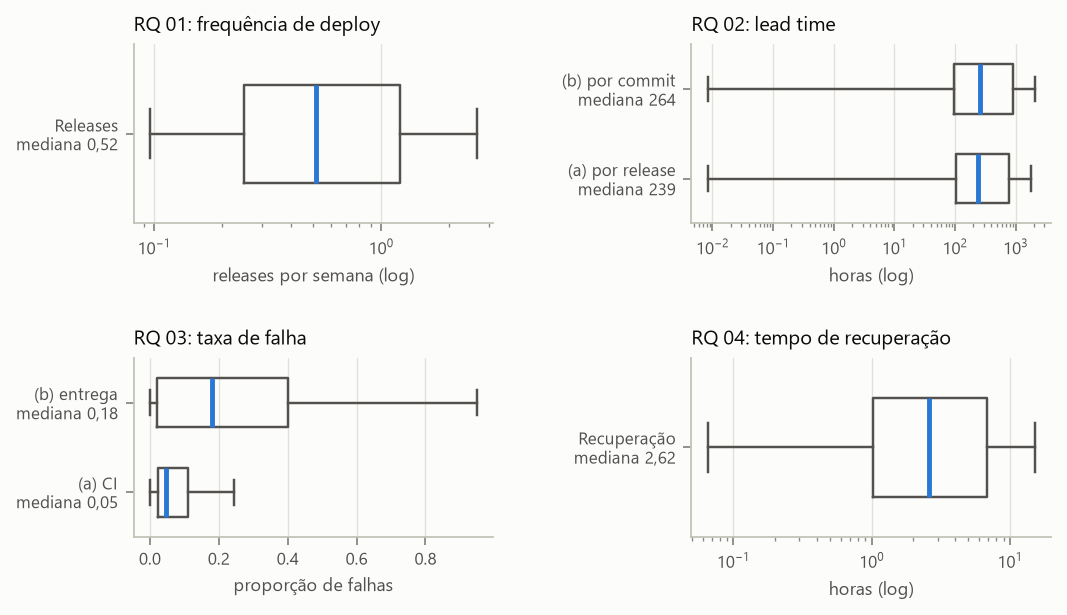
\includegraphics[width=0.9\linewidth]{figuras/rq01_04_painel.png}
\caption{RQ 01 a 04: caixa = IQR, linha azul = mediana, bigodes = 1,5 $\times$ IQR (extremos omitidos); escala logarítmica, exceto no CFR.}
\label{fig:rq0104}
\end{figure}

\subsection{RQ 05: frequência de deploy e taxa de falha}
\label{sec:rq05}

A correlação de Spearman entre a frequência e o CFR é positiva e fraca com o CFR de CI ($\rho=0{,}15$; $p=0{,}008$; $n=300$) e positiva e moderada com o de entrega ($\rho=0{,}48$; $p<0{,}001$; $n=298$), na Figura~\ref{fig:rq05}. Com o CFR de CI, 89\% dos repositórios ficam abaixo de 20\% qualquer que seja a frequência, o que é compatível com a tese do DORA (sem \emph{trade-off}), mas não mostra que os mais rápidos sejam mais estáveis. O aumento do CFR (b) é em boa parte efeito do proxy: quem publica várias vezes por semana tem mais chance de um \emph{patch} em até 7 dias, e a mediana do CFR (b) vai de 0 no primeiro quartil de frequência a cerca de 0,33 no último. A tendência cai acima de 3 releases por semana, mas só 31 repositórios estão nessa faixa (4 acima de 10), e não a tratamos como resultado.

\begin{figure}[!t]
\centering
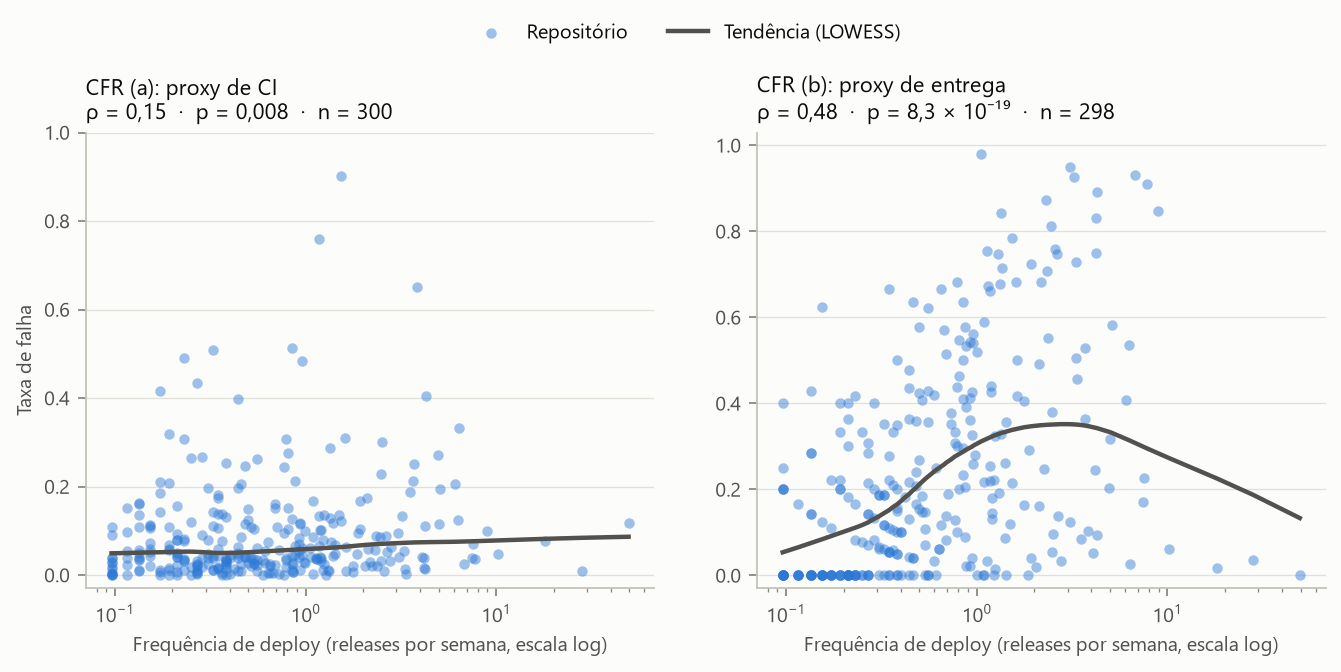
\includegraphics[width=0.95\linewidth]{figuras/rq05_dispersao_compacta.png}
\caption{Frequência de deploy (escala log) e CFR, com a tendência LOWESS.}
\label{fig:rq05}
\end{figure}

\subsection{RQ 06: características associadas ao desempenho}
\label{sec:rq06}

Comparamos as seis métricas entre cinco fatores: linguagem (as com menos de 10 repositórios em ``Outras''), estrelas, contribuidores e idade (quartis) e tipo do projeto (só os 60 rotulados). Todos têm quatro ou mais grupos, e usamos Kruskal-Wallis~\cite{kruskal1952}, $\varepsilon^2=H/(n-1)$ como tamanho de efeito~\cite{tomczak2014} e a correção de Holm~\cite{holm1979} nos 30 $p$-valores; as faixas de $\varepsilon^2$ ($<0{,}01$ desprezível, $<0{,}04$ pequeno, $<0{,}16$ médio, o resto grande) são convenção nossa. Dez testes seguem significativos (Figura~\ref{fig:rq06}). A idade tem efeito grande sobre o lead time ($\varepsilon^2$ de 0,31 e 0,28) e o CFR (b) (0,18) e médio sobre a frequência (0,10): do quartil mais novo ao mais antigo, o lead time (a) mediano vai de 83 h a 721 h, a frequência cai de 0,88 a 0,36 releases por semana e o CFR (b) cai de 0,32 a 0,03. Contribuidores têm efeito médio sobre o lead time (149 h no quartil com menos contribuidores, 440 h no com mais) e o CFR (b); a linguagem, sobre o lead time (de 156 h em Python e 173 h em TypeScript a 1.119 h em C++) e o CFR (b). Estrelas e tipo do projeto não foram significativos, e os outros 20 testes têm $\varepsilon^2\leq 0{,}12$.

\begin{figure}[!t]
\centering
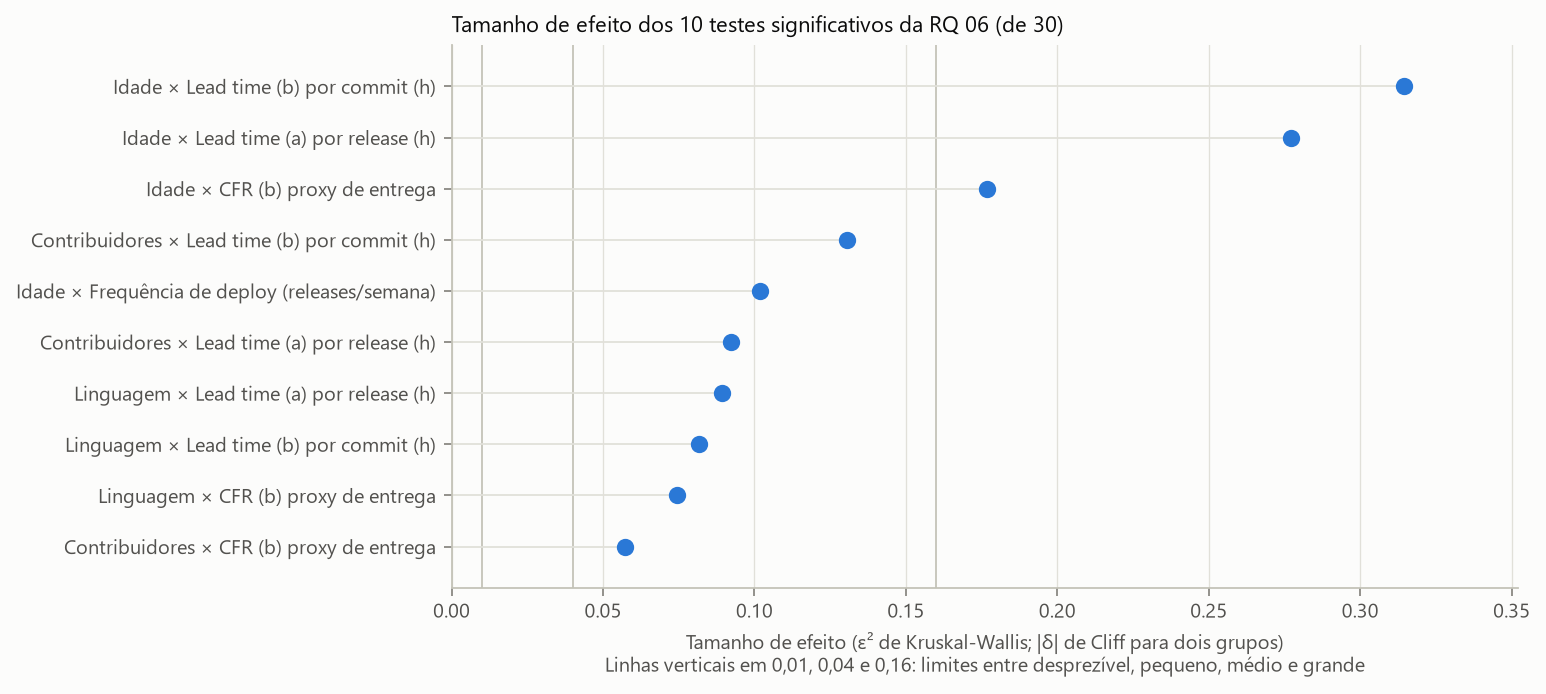
\includegraphics[width=0.95\linewidth]{figuras/rq06_efeitos_significativos.png}
\caption{Tamanho de efeito dos testes significativos após Holm; linhas em 0,01, 0,04 e 0,16.}
\label{fig:rq06}
\end{figure}

\subsection{RQ 07 e RQ 08: sensibilidade e \emph{rework rate}}
\label{sec:rq07}

A Tabela~\ref{tab:rq07} compara C1, C2 e C3 (Seção~\ref{sec:definicoes}); a recuperação é a mesma nas três, e 15 a 17 repositórios ficam sem classificação geral em cada uma. De 23,7\% a 26,1\% mudam de categoria geral, menos que os 30\% previstos, com kappa ponderado de 0,58 a 0,65 e 93\% a 97\% das mudanças entre vizinhas. Essa estabilidade esconde mudanças grandes por métrica: a faixa de lead time muda em cerca de metade dos repositórios, e a de CFR em 54\% quando o proxy de entrega entra; a geral muda menos por ser a mediana de quatro notas, com a recuperação como âncora. As alternativas deslocam a classificação em sentidos opostos: tags (C3) a melhoram (54 sobem, 15 descem), pois muitos projetos criam tags sem release (uma por pacote em monorepos), elevando a frequência mediana de 0,52 a 0,90; pré-releases e o proxy de entrega (C2) a pioram (45 descem, 29 sobem), sobretudo pelo CFR, cuja mediana vai de 4,6\% a 15,2\%. Cada combinação muda mais de uma definição, então não atribuímos uma mudança a uma única escolha: a classificação geral é moderadamente robusta, mas as conclusões por métrica dependem da variante.

\textbf{RQ 08 (bônus).} A \emph{rework rate}, fração de releases corretivas pela mesma heurística, tem mediana de 0,60 [0,33; 0,80], contra 0,18 [0,02; 0,40] do CFR (b), e o supera em 263 de 298 repositórios (88\%), com correlação fraca ($\rho=0{,}32$). Em projetos com \emph{Conventional Commits}, quase toda release de \emph{patch} tem um commit \texttt{fix:}, e a taxa passa a medir a proporção de releases de \emph{patch}, um traço do versionamento, e não o retrabalho do DORA.

\begin{table}[!t]
\centering
\footnotesize
\setlength{\tabcolsep}{2.5pt}
\caption{RQ 07. Em cima, mediana [IQR] e categoria geral (Elite/High/Medium/Low/sem). Embaixo, mudança entre combinações.}
\label{tab:rq07}
\begin{tabular}{lrcccc}
\toprule
 & Unid. & Frequência & Lead time (h) & CFR & E/H/M/L/sem \\
\midrule
C1 & 22.005 & 0,52 [0,25; 1,21] & 239 [103; 796] & 0,046 [0,023; 0,112] & 20/122/130/12/16 \\
C2 & 28.454 & 0,65 [0,31; 1,38] & 194 [74; 531]  & 0,152 [0,018; 0,354] & 10/118/145/10/17 \\
C3 & 51.392 & 0,90 [0,36; 2,16] & 183 [72; 486]  & 0,046 [0,023; 0,112] & 24/150/105/6/15 \\
\midrule
\multicolumn{6}{l}{\emph{Par: $n$; mudam de categoria; sobem/descem; $\kappa$ ponderado; mudança de faixa em freq./lead time/CFR}} \\
C1$\times$C2 & 283 & 74 (26,1\%) & 29/45 & 0,580 & 11,3\% / 46,5\% / 54,0\% \\
C1$\times$C3 & 284 & 69 (24,3\%) & 54/15 & 0,645 & 25,7\% / 49,5\% / 0,0\% \\
C2$\times$C3 & 283 & 67 (23,7\%) & 63/4  & 0,639 & 14,7\% / 13,0\% / 54,0\% \\
\bottomrule
\end{tabular}
\end{table}

\section{Discussão}
\label{sec:discussao}

A Tabela~\ref{tab:hipoteses} confronta as hipóteses com os resultados. Três deles contrariaram a intuição. Primeiro, projetos com mais contribuidores têm lead time \emph{maior}, e não menor, o que sugere um processo de release mais cauteloso nos projetos grandes (hipótese não testada). Segundo, a correlação entre frequência e CFR de entrega foi mais forte que a prevista, e a RQ 07 e a RQ 08 apontam a mesma causa: o proxy de release corretiva mede em boa parte a política de versionamento. Terceiro, a mediana do lead time por release (a) ficou \emph{abaixo} da por commit (b), ao contrário do previsto, embora (a) seja maior em 178 de 299 repositórios, pois a diferença entre medianas não é a comparação pareada.

\begin{table}[!t]
\centering
\footnotesize
\setlength{\tabcolsep}{3pt}
\caption{Hipóteses frente aos resultados.}
\label{tab:hipoteses}
\begin{tabular}{>{\raggedright\arraybackslash}p{0.8cm}>{\raggedright\arraybackslash}p{11.9cm}>{\raggedright\arraybackslash}p{2.3cm}}
\toprule
 & Resultado & Situação \\
\midrule
H1 & Mediana de 0,518 releases/semana; \emph{Medium} em 137 de 300 (45,7\%), sem maioria absoluta. & Em parte \\
H2 & Medianas de 239 h (a) e 264 h (b); (a) supera (b) em 178 de 299 e fica acima de 30 dias em 80. & Em parte \\
H3 & Medianas de 4,6\% (CI) e 18,1\% (entrega), fora das faixas previstas; $\rho=0{,}13$ entre os proxies. & Em parte \\
H4 & Mediana de 2,6 h, cauda até 182 h e 0,47\% de episódios censurados. & Compatível em parte \\
H5 & CFR (a): $\rho=0{,}15$, fraca mas positiva; CFR (b): $\rho=0{,}48$, mais forte que o previsto. & Em parte \\
H6 & (i) refutada: lead time maior com mais contribuidores; (ii) inconclusiva (60 repositórios); (iii) refutada: frequência sem diferença após Holm; (iv) confirmada ($\varepsilon^2=0{,}31$). & 1 de 4 confirmada \\
H7 & 24\% a 26\% mudam de categoria; $\kappa$ de 0,58 a 0,65; 93\% a 97\% entre vizinhas. & Em parte \\
H8 & \emph{Rework rate} maior que o CFR (b) em 88\%, mas 0,60 contra 0,18 e $\rho=0{,}32$. & Em parte \\
\bottomrule
\end{tabular}
\end{table}

\section{Ameaças à validade}
\label{sec:ameacas}

Seguimos as quatro categorias clássicas~\cite{wohlin2012}. \textbf{Construto:} uma release não é um deploy (na validação, a concordância sobre entrega real foi de 87\% em média entre pares, e os três coincidiram em 80\% dos repositórios), e por isso lemos a frequência como publicação de versões; uma falha de CI não é uma falha em produção; o CFR (b) depende de uma heurística cujo F1 variou de 0,56 a 0,76 conforme a referência e está acoplado à frequência; a recuperação por CI conta uma nova execução do mesmo commit como recuperação; e a data de autoria preserva a data original em \emph{rebases} e pode inflar o lead time. \textbf{Interna:} a idade se associa a quase todas as métricas e as comparações são univariadas, então não isolam seu efeito; cada combinação da RQ 07 muda mais de uma definição; e a rotulagem não teve calibração prévia (para preservar a independência), o que deixou limiares diferentes para ``objetivo principal'', além de o número da versão, visível no nome da release, poder influenciar o julgamento. \textbf{Externa:} a amostra reúne 300 repositórios muito populares (mediana de 62 mil estrelas), com Actions, escolhidos em ordem decrescente de estrelas, e não se estende a projetos corporativos, pequenos ou com outro CI; a validação cobre 60 repositórios, sorteados de um subconjunto de 100. \textbf{Conclusão:} foram 30 testes com correção de Holm, e resultados com $p$ ajustado próximo de 0,05 (CFR (b) por linguagem, $p=0{,}024$) são frágeis; há grupos pequenos (14 repositórios em C++; 8 a 24 por tipo de projeto); o kappa de entrega real é baixo em parte pela prevalência; e a robustez da classificação geral é em parte efeito da mediana de quatro notas.

\section{Replicação cruzada}
\label{sec:replicacao}

Não realizamos a replicação cruzada neste ciclo, por falta de tempo, e não recebemos Issues de replicação de outro grupo até o fechamento deste texto. Para facilitar a replicação do nosso estudo, o pipeline roda com um único comando documentado no README, com cache e retomada, e o repositório inclui o script \texttt{analises/replicacao.py}, que compara um CSV replicado com o original (diferença relativa por métrica e concordância da classificação DORA), com testes automatizados.

\section{Conclusão}
\label{sec:conclusao}

Calculamos as métricas DORA de 300 repositórios populares por proxies e mostramos que sua leitura depende das definições: a classificação geral é moderadamente robusta (cerca de três em quatro repositórios mantêm a categoria), mas a faixa de cada métrica muda com a variante, e a frequência mede publicação de versões, não deploy em produção. A taxa de falha por entrega cresce com a frequência em boa parte por efeito do proxy, e a idade do repositório é o fator mais associado ao lead time. A heurística de release corretiva tem F1 de 0,73 pelo consenso, mas esse valor depende da referência adotada. As principais limitações são a amostra de repositórios muito populares, a rotulagem sem calibração e a ausência de replicação por outro grupo. Com mais tempo, expandiríamos a validação manual para mais repositórios e testaríamos modelos multivariados para separar o efeito da idade.

\section*{Disponibilidade}
Repositório: \url{https://github.com/gsantss/lab03-dora-metrics}. Quadro de trabalho: \url{https://github.com/users/gsantss/projects/8}.

\bibliographystyle{sbc}
\bibliography{referencias}

\end{document}
